\documentclass{standalone}
\usepackage{times}
\usepackage{mathtools}

\usepackage{tikz}
\usetikzlibrary{positioning,fit,shapes,calc,decorations.pathreplacing}
\usetikzlibrary{backgrounds}
\usetikzlibrary{arrows.meta}
\usetikzlibrary{shapes,snakes}

\definecolor{processblue}{cmyk}{1,1,1,0}
\definecolor{accent}{rgb}{0.6,0.6,0.6}
\definecolor{accent2}{rgb}{0.9,0.9,0.9}


\definecolor{myblue}{rgb}{0.0,0.5,0.8}

\begin{document}
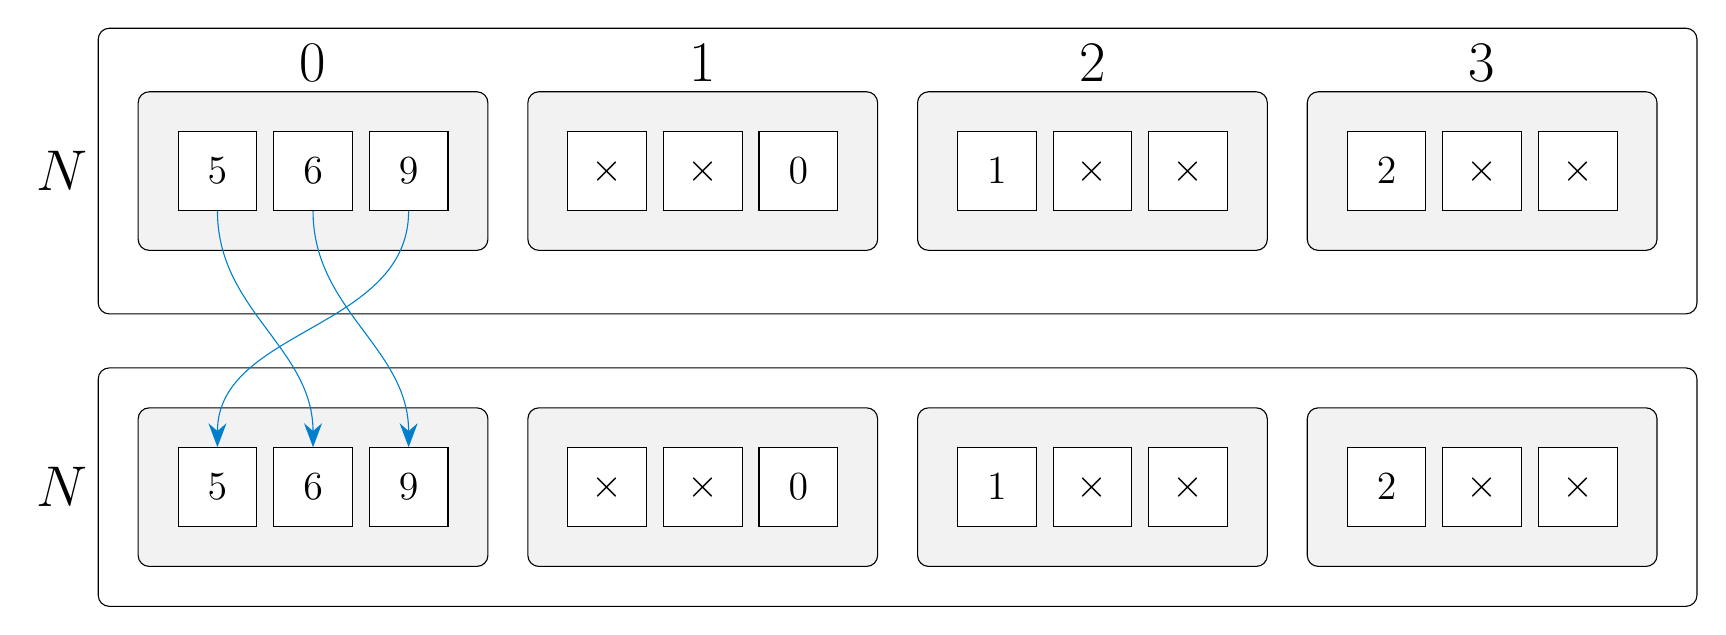
\begin{tikzpicture}[
  data/.style = {
    draw,
    rectangle,
    fill = white,
    minimum width = 1.0cm,
    minimum height = 1.0cm,
  },
  next/.style = {
    draw,
    circle,
    fill=black,
  },
  edge/.style = {
    draw,
    rectangle,
    rounded corners,
    minimum width = 0.5cm,
    minimum height = 0.5cm,
  },
  vedge/.style = {
    edge,
    top color = black!5,
    bottom color = black!5,
  },
  fedge/.style = {
    edge,
    top color = accent,
    bottom color = accent,
  },
  >={Stealth[scale=1.8]},
]

  %
  \node[data] (n00) {\Large $5$};
  \node[data] (n01) [right=0.2cm of n00] {\Large $6$};
  \node[data] (n02) [right=0.2cm of n01] {\Large $9$};
  \begin{scope}[on background layer]
    \node[vedge,fit=(n00) (n02),inner sep=0.5cm,label={above: \huge $0$}] (n0) {};
  \end{scope}

  \node[data] (n10) [right=of n0] {\Large $\times$};
  \node[data] (n11) [right=0.2cm of n10] {\Large $\times$};
  \node[data] (n12) [right=0.2cm of n11] {\Large $0$};
  \begin{scope}[on background layer]
    \node[vedge,fit=(n10) (n12),inner sep=0.5cm,label={above: \huge $1$}] (n1) {};
  \end{scope}

  \node[data] (n20) [right=of n1] {\Large $1$};
  \node[data] (n21) [right=0.2cm of n20] {\Large $\times$};
  \node[data] (n22) [right=0.2cm of n21] {\Large $\times$};
  \begin{scope}[on background layer]
    \node[vedge,fit=(n20) (n22),inner sep=0.5cm,label={above: \huge $2$}] (n2) {};
  \end{scope}

  \node[data] (n30) [right=of n2] {\Large $2$};
  \node[data] (n31) [right=0.2cm of n30] {\Large $\times$};
  \node[data] (n32) [right=0.2cm of n31] {\Large $\times$};
  \begin{scope}[on background layer]
    \node[vedge,fit=(n30) (n32),inner sep=0.5cm,label={above: \huge $3$}] (n3) {};
  \end{scope}

  %
  \node[data] (nn00) [below=3cm of n00] {\Large $5$};
  \node[data] (nn01) [right=0.2cm of nn00] {\Large $6$};
  \node[data] (nn02) [right=0.2cm of nn01] {\Large $9$};
  \begin{scope}[on background layer]
    \node[vedge,fit=(nn00) (nn02),inner sep=0.5cm] (nn0) {};
  \end{scope}

  \node[data] (nn10) [right=of nn0] {\Large $\times$};
  \node[data] (nn11) [right=0.2cm of nn10] {\Large $\times$};
  \node[data] (nn12) [right=0.2cm of nn11] {\Large $0$};
  \begin{scope}[on background layer]
    \node[vedge,fit=(nn10) (nn12),inner sep=0.5cm] (nn1) {};
  \end{scope}

  \node[data] (nn20) [right=of nn1] {\Large $1$};
  \node[data] (nn21) [right=0.2cm of nn20] {\Large $\times$};
  \node[data] (nn22) [right=0.2cm of nn21] {\Large $\times$};
  \begin{scope}[on background layer]
    \node[vedge,fit=(nn20) (nn22),inner sep=0.5cm] (nn2) {};
  \end{scope}

  \node[data] (nn30) [right=of nn2] {\Large $2$};
  \node[data] (nn31) [right=0.2cm of nn30] {\Large $\times$};
  \node[data] (nn32) [right=0.2cm of nn31] {\Large $\times$};
  \begin{scope}[on background layer]
    \node[vedge,fit=(nn30) (nn32),inner sep=0.5cm] (nn3) {};
  \end{scope}

  \begin{scope}[on background layer]
    % \node[vedge,fit=(v0) (v7),label={left: \huge $v$},inner sep=0.5cm,inner ysep=0.8cm] (v) {};
    \node[edge,fit=(n0) (n3),label={left:\huge $N$},inner sep=0.5cm,inner ysep=0.8cm] (n) {};
    \node[edge,fit=(nn0) (nn3),label={left:\huge $N$},inner sep=0.5cm] (nn) {};
  \end{scope}

  \path[->,myblue] (n00) edge[out=-90,in=90] node {} (nn01);
  \path[->,myblue] (n01) edge[out=-90,in=90] node {} (nn02);
  \path[->,myblue] (n02) edge[out=-90,in=90] node {} (nn00);

\end{tikzpicture}
\end{document}
